% middleware_components.tex
% Auto-generated LaTeX description of middleware modules: core, facade, orchestrator
\documentclass[11pt,a4paper]{article}
\usepackage[utf8]{inputenc}
\usepackage[T1]{fontenc}
\usepackage{lmodern}
\usepackage{microtype}
\usepackage{geometry}
\geometry{margin=1in}
\usepackage{hyperref}
\usepackage{listings}
\usepackage{xcolor}
\usepackage{parskip}
\usepackage{tikz}
\usetikzlibrary{arrows.meta, positioning, shapes.multipart, calc}

% Listings style for Python
\lstdefinestyle{pythonstyle}{
  language=Python,
  basicstyle=\ttfamily\small,
  keywordstyle=\color{blue},
  stringstyle=\color{orange},
  commentstyle=\color{gray},
  breaklines=true,
  frame=single,
  tabsize=2,
  showstringspaces=false
}

\title{Architecture and Components of the Digital Twins Middleware}
\author{Auto-generated from repository analysis}
\date{\today}

\begin{document}
\maketitle
\begin{abstract}
This document summarizes the structure and runtime behavior of the middleware for digital twins implemented in the repository. It describes the responsibilities of the three main modules: \texttt{core}, \texttt{facade}, and \texttt{orchestrator}. Code excerpts and a component interaction figure are included to help explain the flows.
\end{abstract}

\section{Overview}
The middleware organizes concerns into three main Python/Django modules:
\begin{itemize}
  \item \textbf{core}: configuration and lightweight infrastructure (gateway credentials, DTDL parser client, small auth helpers).
  \item \textbf{facade}: device-facing adapter layer. Models devices and properties, implements RPC calls to ThingsBoard, telemetry formatting (InfluxDB), discovery and session management.
  \item \textbf{orchestrator}: digital-twin model management. Parses DTDL models, materializes Digital Twin Instances, and performs semantic binding between DT properties and device properties.
\end{itemize}

\section{core}
\subsection{Responsibilities}
The \texttt{core} module stores external endpoint configuration and exposes small helper APIs. Two main models are \texttt{GatewayIOT} and \texttt{DTDLParserClient}. It implements a helper to fetch a JWT token from a ThingsBoard gateway which other modules reuse.

\subsection{Example code}
\begin{lstlisting}[style=pythonstyle,caption={JWT acquisition helper (simplified) from \texttt{core/api.py}}]
@router.get("/gatewayiot/{gateway_id}/jwt/")
def get_jwt_token_gateway(request, gateway_id: int):
    gateway = get_object_or_404(GatewayIOT, id=gateway_id)
    url = f"{gateway.url}/api/auth/login"
    payload = {"username": gateway.username, "password": gateway.password}
    response = requests.post(url, json=payload)
    if response.status_code == 200:
        return {"token": response.json().get("token")}, 200
    return {"error": "Error obtaining JWT token"}, 400
\end{lstlisting}

\section{facade}
\subsection{Responsibilities}
The \texttt{facade} module encapsulates interactions with ThingsBoard and time-series storage (InfluxDB). It models \texttt{Device}, \texttt{Property}, and \texttt{DeviceType}. Responsibilities include:
\begin{itemize}
  \item Discovering devices via ThingsBoard and creating/updating local \texttt{Device} rows.
  \item Performing RPC calls to devices with aggressive timeouts for low latency and a fallback strategy.
  \item Formatting telemetry into InfluxDB line protocol and sending points.
  \item Managing HTTP sessions optimized for reduced latency.
\end{itemize}

\subsection{Example code}
\begin{lstlisting}[style=pythonstyle,caption={Ultra-fast RPC call excerpt (simplified) from \texttt{facade/models.py}}]
def call_rpc(self, rpc_type: RPCCallTypes):
    # obtain JWT
    response, status_code = get_jwt_token_gateway(None, gateway.id)
    if status_code != 200:
        return self._create_mock_response()
    token = response['token']
    urltwoway = f"{gateway.url}/api/rpc/twoway/{device.identifier}"
    session = get_session_for_gateway(gateway.id)
    response = session.post(urltwoway,
                             json={"method": self.rpc_write_method, "params": self.get_value()},
                             headers={"X-Authorization": f"Bearer {token}"},
                             timeout=current_timeout)
    return response
\end{lstlisting}

\subsection{Telemetry helper}
The repository centralizes InfluxDB line-protocol formatting in a utility function to avoid inconsistencies across the codebase.
\begin{lstlisting}[style=pythonstyle,caption={Influx line-protocol formatter (simplified) from \texttt{facade/utils.py}}]
def format_influx_line(measurement, tags: dict, fields: dict, timestamp=None):
    # escape tags and format field values (booleans/ints -> floats)
    # return single line string in InfluxDB line protocol
    return f"...line protocol..."
\end{lstlisting}

\section{orchestrator}
\subsection{Responsibilities}
The \texttt{orchestrator} module handles the transformation of DTDL model specifications into runtime entities (models, elements, relationships) and the creation of \texttt{DigitalTwinInstance}s. It also contains logic for mapping DT properties to physical device properties using semantic similarity embeddings.

\subsection{Example code}
\begin{lstlisting}[style=pythonstyle,caption={DTDL parsing and parsed specification retrieval (simplified) from \texttt{orchestrator/models.py}}]
def create_parsed_specification(self):
    parser_client = DTDLParserClient.get_active()
    response = requests.post(parser_client.url, json={"id": self.specification.get('@id'),
                                                      "specification": self.specification})
    response.raise_for_status()
    self.parsed_specification = response.json()
\end{lstlisting}

\subsection{Semantic binding}
The orchestrator uses a sentence-transformer model to compute embeddings for DT properties and candidate device properties; it then picks the best match if the similarity exceeds a threshold (e.g., 0.60).
\begin{lstlisting}[style=pythonstyle,caption={Semantic binding sketch from \texttt{orchestrator/models.py}}]
from sentence_transformers import SentenceTransformer, util
model = SentenceTransformer("all-MiniLM-L6-v2")
dt_embedding = model.encode(dt_text, convert_to_tensor=True)
# compare against device embeddings
score = float(util.cos_sim(dt_embedding, device_embedding)[0][0])
if score >= 0.60:
    self.device_property = best_match
\end{lstlisting}

\section{Interaction figure}
The following figure summarizes the typical runtime interaction between modules. It covers: device discovery, DTDL parsing and instance creation, and DT property propagation to devices.

\begin{figure}[h!]
\centering
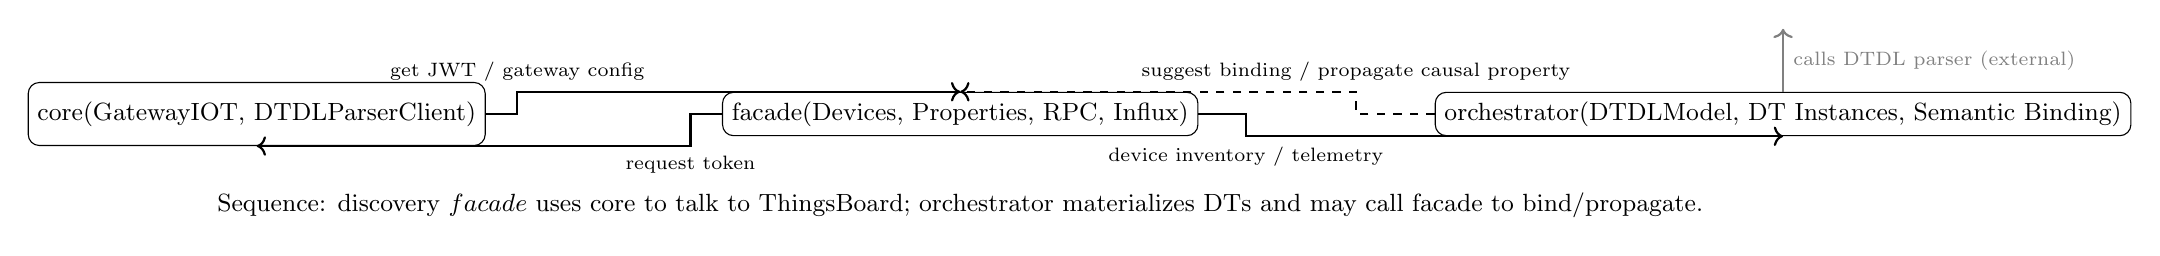
\begin{tikzpicture}[node distance=18mm, every node/.style={font=\small}]
  % nodes
  \node[draw, rectangle, rounded corners, minimum width=30mm, minimum height=8mm] (core) {core\n(GatewayIOT, DTDLParserClient)};
  \node[draw, rectangle, rounded corners, right=30mm of core, minimum width=30mm] (facade) {facade\n(Devices, Properties, RPC, Influx)};
  \node[draw, rectangle, rounded corners, right=30mm of facade, minimum width=30mm] (orchestrator) {orchestrator\n(DTDLModel, DT Instances, Semantic Binding)};

  % arrows
  \draw[->, thick] (core.east) -- ++(4mm,0) |- (facade.north) node[midway, above, font=\scriptsize] {get JWT / gateway config};
  \draw[->, thick] (facade.west) -- ++(-4mm,0) |- (core.south) node[midway, below, font=\scriptsize] {request token};

  \draw[->, thick] (facade.east) -- ++(6mm,0) |- (orchestrator.south) node[midway, below, font=\scriptsize] {device inventory / telemetry};
  \draw[->, thick, dashed] (orchestrator.west) -- ++(-10mm,0) |- (facade.north) node[midway, above, font=\scriptsize] {suggest binding / propagate causal property};

  \draw[->, thick, color=gray] (orchestrator.north) -- ++(0,8mm) node[midway, right, font=\scriptsize] {calls DTDL parser (external)};

  % annotations
  \node[below=6mm of facade] (note) {Sequence: discovery \(facade\) uses core to talk to ThingsBoard; orchestrator materializes DTs and may call facade to bind/propagate.};
\end{tikzpicture}
\caption{Module interactions: token acquisition, device discovery, DT creation and property propagation.}
\end{figure}

\subsection{Figure explanation}
The figure shows three primary modules laid out left-to-right. Typical flows:
\begin{enumerate}
  \item Core stores gateway credentials and DTDL parser endpoints. When \texttt{facade} needs to talk to ThingsBoard it first requests a JWT token from \texttt{core} utilities.
  \item Facade performs discovery and populates the local devices database. It also issues RPC calls for reads/writes and writes telemetry points to InfluxDB.
  \item Orchestrator parses DTDL (via an external parser), creates model elements and hierarchical instances. It then suggests device-property bindings by comparing embeddings. For causal DT properties bound to devices, orchestrator triggers propagation which flows back through \texttt{facade} to call RPCs on the device.
\end{enumerate}

\section{Notes and recommended experiments}
A few practical items to discuss in the article:
\begin{itemize}
  \item Evaluate timeout vs accuracy trade-offs in the RPC path (facade). The code uses ultra-low timeouts and fallback mocked responses for availability.
  \item Measure semantic-binding precision and consider a human-in-the-loop confirmation step to avoid incorrect automatic bindings.
  \item Consider instrumenting counts/metrics for parser failures, fallback RPCs, and binding acceptance rates.
\end{itemize}

\section{Appendix: small glossary}
\begin{itemize}
  \item DTDL: Digital Twins Definition Language.
  \item DT: Digital Twin.
  \item RPC: Remote Procedure Call (ThingsBoard RPC endpoints used to command/read devices).
  \item InfluxDB: time-series storage used for telemetry and inactivity events.
\end{itemize}

\end{document}
